% Copyright 2026 Sreeram Anil
% SPDX-License-Identifier: CC-BY-4.0
% =============================================================================
%  Cubature Kalman filter (third degree) — classical Kalman family
% =============================================================================
\chapter{Cubature Kalman Filter (CKF)}
\label{ch:ckf}

\section*{At a glance}
\begin{tabular}{@{}l>{\raggedright\arraybackslash}p{0.76\textwidth}@{}}
Family & classical Kalman (sigma-point) \\
Header & \texttt{include/estkit/filters/ckf.hpp} \\
Registered name & \texttt{CKF} \\
State dimension & $n_x = 4$ (cell model) --- generic in $n_x, n_u, n_y$ \\
Cubature points & $2n_x = 8$, equal weights $1/2n_x$, no tuning parameters \\
Cost per step & $\mathcal{O}(n_x^3)$ plus $4n_x$ model calls; $1.18$--$1.26\,\SI{}{\micro\second}$/step \\
Primary references & \cite{arasaratnam2009ckf,ito2000gaussian,sarkka2013} \\
\end{tabular}

\section{Motivation and aerospace/BMS relevance}
The unscented transform has three free parameters ($\alpha,\beta,\kappa$) whose ``correct''
values are the subject of a large and not always consistent literature, and for $n_x>3$ the
canonical choice $\kappa = 3-n_x$ makes the centre weight negative, so the transformed
covariance can lose positive definiteness. Arasaratnam and Haykin~\cite{arasaratnam2009ckf}
removed both problems by asking a different question: instead of designing a point set to
match moments, derive the numerically optimal cubature rule for the specific integral that a
Gaussian filter has to evaluate. The answer --- the third-degree spherical-radial rule --- is
parameter-free, has $2n_x$ points of \emph{equal positive} weight $1/(2n_x)$, and therefore
always produces a positive semi-definite covariance.

That combination (no tuning, guaranteed definiteness, derivative-free) is attractive for
certified software: there is no parameter for a reviewer to question and no failure branch to
justify. The CKF has become the default sigma-point filter in a large part of the aerospace
navigation literature for exactly this reason, and it is the natural baseline for the
square-root (Chapter~\ref{ch:sckf}) and fifth-degree (Chapter~\ref{ch:ckf5}) variants.

\section{Problem statement and assumptions}
Model \eqref{eq:ekf-proc}--\eqref{eq:ekf-meas} with additive noise. The Gaussian
(assumed-density) filter requires, at every step, integrals of the form
\begin{equation}
I[g] = \int_{\real^{n_x}} g(\vx)\, \N{\vx;\xhat}{\mP}\, d\vx,
\label{eq:ckf-integral}
\end{equation}
with $g$ ranging over $f$, $h$ and the outer products $ff^\T$, $hh^\T$ and $\vx h^\T$. No
differentiability of $g$ is needed --- only that the integrals exist. As for the UKF, the
filtering density is assumed to be adequately described by its first two moments.

\section{Derivation}
\paragraph{Spherical-radial decomposition.} Substituting $\vx = \xhat + \mS\vz$ with
$\mS\mS^\T = \mP$ turns \eqref{eq:ckf-integral} into a standard-Gaussian integral, and then
$\vz = r\bm{u}$ with $\norm{\bm{u}}=1$, $r\ge0$, splits it into a radial and a spherical
part:
\begin{equation}
I[g] = \frac{1}{(2\pi)^{n_x/2}}\int_0^\infty\!\!\int_{U_{n_x}} g(\xhat + \mS r\bm{u})\,
 r^{n_x-1}e^{-r^2/2}\,d\sigma(\bm{u})\,dr,
\label{eq:ckf-sr}
\end{equation}
where $U_{n_x}=\{\bm{u}: \bm{u}^\T\bm{u}=1\}$ and $\sigma$ is the spherical surface measure.
Arasaratnam and Haykin treat the two factors separately: the spherical integral by the
third-degree rule of Stroud~\cite{stroud1971}, which uses the $2n_x$ intersections of the
unit sphere with the coordinate axes and equal weights, and the radial integral --- after the
substitution $t = r^2/2$ a Gamma-weighted integral --- by the first-order Gauss--Laguerre
rule, which places a single node at $t = n_x/2$, i.e. $r = \sqrt{n_x}$. Combining the two,
\begin{equation}
I[g] \approx \frac{1}{2n_x}\sum_{i=1}^{2n_x} g\!\left(\xhat + \mS\,\bm{\xi}_i\right),
\qquad
\bm{\xi}_i = \sqrt{n_x}\,[\bm{1}]_i,
\label{eq:ckf-rule}
\end{equation}
where $[\bm{1}]_i$ runs over the $2n_x$ columns of $[\,\mI_{n_x}\; -\mI_{n_x}\,]$. The rule is
\emph{exact} for every monomial in $\vz$ of total degree $\le 3$: the zeroth moment gives
$\sum w_i = 1$, the second gives $\frac{1}{2n_x}\cdot 2\cdot n_x = 1$ per coordinate, and all
odd moments vanish by the central symmetry of the point set. It is not exact at degree four
($\sum w_i \xi_{i1}^4 = n_x$ versus the true value $3$), which is the source of the
differences with the fifth-degree rules discussed in Chapter~\ref{ch:ckf5}.

\begin{remark}[Relation to the UKF]
Setting $\alpha = 1$, $\kappa = 0$ in \eqref{eq:ukf-lambda} gives $\lambda = 0$,
$W_0^m = 0$, $W_{i} = 1/(2n_x)$ and points at $\pm\sqrt{n_x}$ standard deviations: the CKF is
exactly the scaled unscented transform with $\lambda = 0$ plus the deletion of the (zero
mean-weight) centre point. We used this identity as a cross-check: with $\alpha=1,\kappa=0$
the library UKF reproduces the CKF's benchmark behaviour on every scenario, which validates
both implementations.
\end{remark}

\paragraph{Filter recursion.} With $\mS^+ = \operatorname{chol}(\Pplus_{k-1})$,
\begin{align}
\mathcal{X}_i &= \xplus_{k-1} + \sqrt{n_x}\,\mS^+[\bm{1}]_i, &
\mathcal{X}^*_i &= f(\mathcal{X}_i,\vu_{k-1}), \label{eq:ckf-tu1}\\
\xminus_k &= \frac{1}{2n_x}\sum_i \mathcal{X}^*_i, &
\Pminus_k &= \frac{1}{2n_x}\sum_i(\mathcal{X}^*_i-\xminus_k)(\mathcal{X}^*_i-\xminus_k)^\T + \mQ,
\label{eq:ckf-tu2}
\end{align}
and, after regenerating the points from $(\xminus_k,\Pminus_k)$,
\begin{align}
\mathcal{Z}_i &= h(\mathcal{X}_i,\vu_k), \qquad \yhat_k = \frac{1}{2n_x}\sum_i \mathcal{Z}_i,
\label{eq:ckf-mu1}\\
\mP_{zz} &= \frac{1}{2n_x}\sum_i(\mathcal{Z}_i-\yhat_k)(\mathcal{Z}_i-\yhat_k)^\T + \mR,
\qquad
\mP_{xz} = \frac{1}{2n_x}\sum_i(\mathcal{X}_i-\xminus_k)(\mathcal{Z}_i-\yhat_k)^\T,
\label{eq:ckf-mu2}\\
\mW_k &= \mP_{xz}\mP_{zz}\inv, \quad
\xplus_k = \xminus_k + \mW_k(\vy_k-\yhat_k), \quad
\Pplus_k = \Pminus_k - \mW_k\mP_{zz}\mW_k^\T.
\label{eq:ckf-mu3}
\end{align}
The original paper writes the covariances as raw second moments minus the outer product of
the means; the implementation accumulates the centred deviations directly, which is
algebraically identical and avoids the cancellation $\overline{XX^\T}-\xhat\xhat^\T$ when the
mean is much larger than the spread --- relevant here, where $\soc\approx 1$ and
$\sigma_\soc\approx 10^{-3}$.

\section{Algorithm}
\begin{algorithm}[H]
\caption{CKF --- one sampling period (additive noise)}
\begin{algorithmic}[1]
\Require $\xplus_{k-1},\Pplus_{k-1},\vu_{k-1},\vy_k,\vu_k$
\State $\mS\gets\operatorname{chol}(\Pplus_{k-1})$;\;
       $\mathcal{X}_{i},\mathcal{X}_{i+n_x}\gets\xplus_{k-1}\pm\sqrt{n_x}\,\mS_{:,i}$, $i=1..n_x$
\State \textbf{Time update:} $\mathcal{X}_i\gets f(\mathcal{X}_i,\vu_{k-1})$;\;
       $\xminus_k\gets\frac{1}{2n_x}\sum_i\mathcal{X}_i$
\State $\Pminus_k\gets\frac{1}{2n_x}\sum_i(\mathcal{X}_i-\xminus_k)(\cdot)^\T+\mQ$; symmetrise
\State \textbf{Regenerate} $\mathcal{X}_i$ from $(\xminus_k,\Pminus_k)$;\;
       $\mathcal{Z}_i\gets h(\mathcal{X}_i,\vu_k)$;\; $\yhat_k\gets\frac{1}{2n_x}\sum_i\mathcal{Z}_i$
\State $\mP_{zz}\gets\frac{1}{2n_x}\sum_i(\mathcal{Z}_i-\yhat_k)(\cdot)^\T+\mR$;\;
       $\mP_{xz}\gets\frac{1}{2n_x}\sum_i(\mathcal{X}_i-\xminus_k)(\mathcal{Z}_i-\yhat_k)^\T$
\State $\mW\gets\mP_{xz}\mP_{zz}\inv$;\; $\xplus_k\gets\xminus_k+\mW(\vy_k-\yhat_k)$;\;
       $\Pplus_k\gets\Pminus_k-\mW\mP_{zz}\mW^\T$
\State \textbf{if} constraints enabled \textbf{then} $\xplus_k\gets\Pi(\xplus_k)$
\Ensure $\xplus_k,\Pplus_k$
\end{algorithmic}
\end{algorithm}

\section{Application to the battery model}
For $n_x=4$ the rule uses eight points at $\pm 2\sigma$ along the principal axes of $\mP$.
With the benchmark's initial covariance ($\sigma_\soc = 0.1$) the SOC points therefore sit at
$\soc_0 \pm 0.2$ --- a $40\,\%$ SOC span over which the NMC/graphite OCV curve is distinctly
non-affine. This is the single most important fact about the CKF on this problem: the
effective (statistical) measurement slope $\mP_{xz}/\mP_{\soc\soc}$ is then the \emph{chord}
of the OCV curve over $[\soc_0-0.2,\soc_0+0.2]$, not the tangent at $\soc_0$.

Options: none. \code{apply\_constraints = true} and \code{q\_scale = r\_scale = 1} are the
only knobs, and they exist for uniformity with the rest of the library, not because the
algorithm needs them.

\section{Implementation notes}
The eight points are stored in a \code{mutable} member array so that
\code{predict\_measurement} --- which the benchmark calls between \code{predict} and
\code{update} --- can regenerate them without copying the filter. The gain uses a direct
$n_y\times n_y$ inverse; for $n_y=1$ that is a division. Guard: if $\mW$ is not finite the
update is skipped and the prior is kept, so a degenerate $\mP_{zz}$ cannot inject NaN into
the state. Memory is 4560\,bytes; the per-step cost, $1.18$--$1.26\,\SI{}{\micro\second}$,
is $\approx 13\,\%$ below the UKF's $1.34$--$1.46$ because there are eight points instead of
nine and no weight arrays. In the single-precision build the results are identical to four decimals and
no covariance lost definiteness --- as guaranteed by the positive weights.

\section{Benchmark results}
\input{tables/cell_CKF.tex}
\begin{figure}[H]\centering
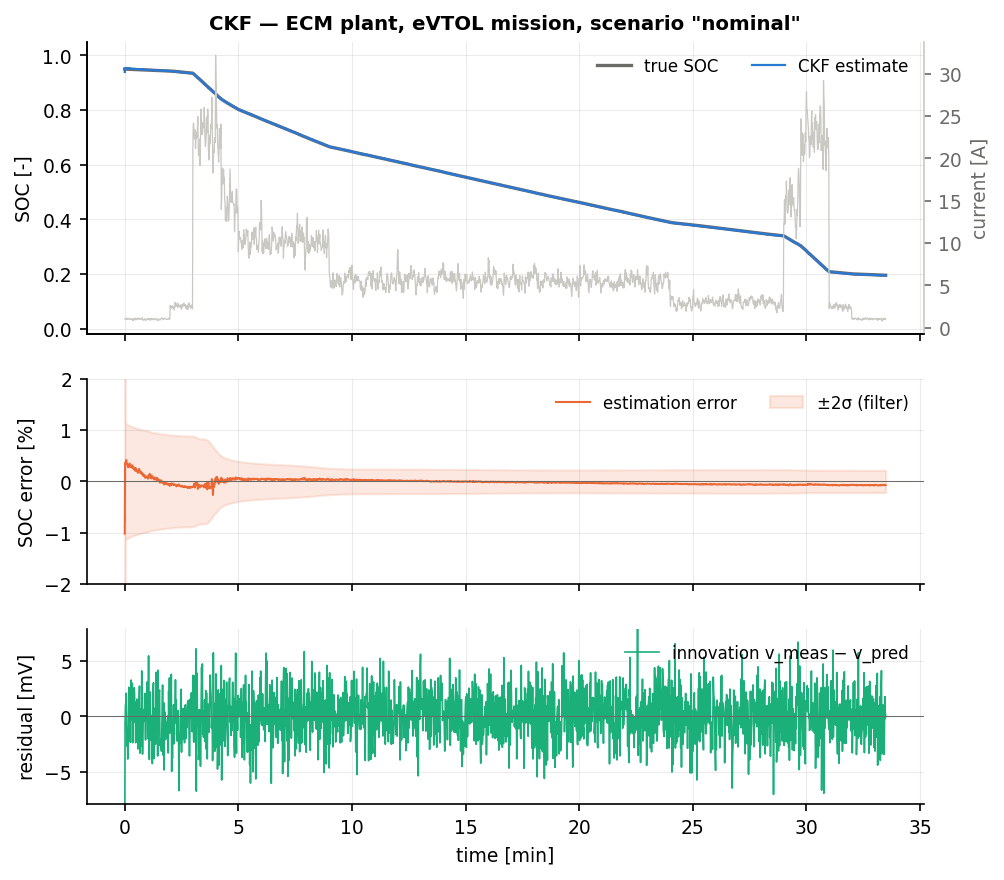
\includegraphics[width=\textwidth]{figures/cell_CKF_nominal.png}
\caption{CKF on the nominal eVTOL mission: true and estimated SOC (top), estimation error with the $\pm 2\sigma$ band when available (middle), voltage residual (bottom).}
\end{figure}
\begin{figure}[H]\centering
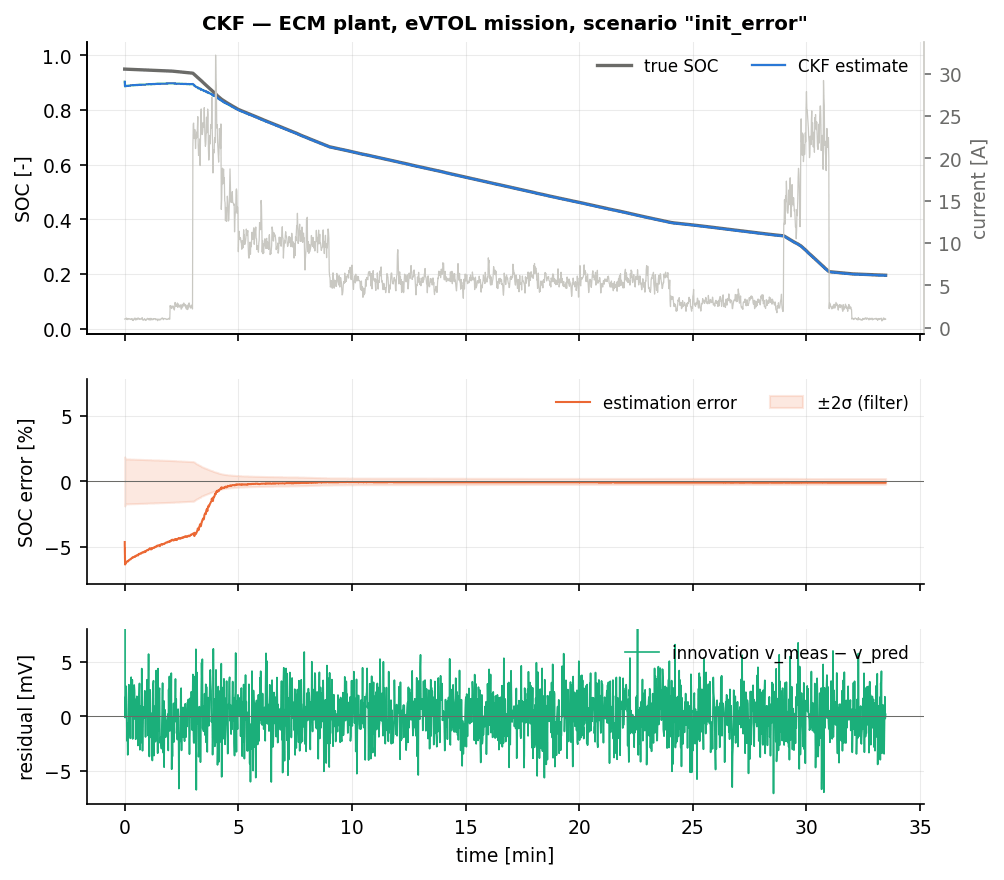
\includegraphics[width=\textwidth]{figures/cell_CKF_init_error.png}
\caption{CKF with a 35\,\% initial SOC error: the $\pm2\sigma$ point spread makes the statistical linearisation use the chord rather than the tangent of the OCV curve, and about $6\,\%$ of the initial error survives the first update.}
\end{figure}

All numbers are three-seed means in per cent SOC.

On \texttt{nominal} the CKF is the most accurate filter in the whole family over the full run:
$\text{RMSE} = 0.08\,\%$ against the EKF's $0.15\,\%$ and the UKF's $0.20\,\%$, with
$\text{RMSE}_{\text{ss}} = 0.05\,\%$ and a maximum error of $1.23\,\%$. It also has the best
\texttt{outliers} figure of the non-robust filters ($0.35/0.07\,\%$ against the EKF's
$0.52/0.21\,\%$), and it wins \texttt{current\_bias} ($0.55\,\%$ against $0.61\,\%$),
\texttt{cold} ($0.11\,\%$ against $0.16\,\%$) and \texttt{hot} is a wash. With a tight prior
the $\pm2\sigma$ points span only a few milli-SOC, the rule is then extremely accurate, and the
equal positive weights give a very clean covariance.

The same $\pm2\sigma$ spread is a liability when the prior is wide. On \texttt{init\_error}
($-35\,\%$) the CKF needs $221$\,s to bring the error below $2\,\%$, against $0$\,s for the EKF
and the UKF, and its whole-run RMSE is $1.64\,\%$ against the EKF's $0.14\,\%$ (the
steady-state value, $0.09\,\%$, is unaffected). The mechanism is the chord effect: with
$\soc_0 = 0.60$ the points sit at $0.40$ and $0.80$, the chord slope over that interval is
$\approx 0.98$\,V while the local slope is $0.80$\,V, so the correction is under-scaled by
$20\,\%$ and about $6\,\%$ of SOC error survives the first update; the prior then collapses and
the residual is removed only slowly by the subsequent small-gain updates. We verified that this
is a property of the point spread and not of the implementation by running the library UKF with
$\alpha = 1,\kappa = 0$ --- the same $\pm\sqrt{n_x}\sigma$ spread --- which reproduces the
behaviour.

The same weakness appears wherever the prior is forced open. \texttt{sensor\_dropout} gives
$2.83/1.92\,\%$ against the EKF's $0.72/0.46\,\%$ and the IEKF's $0.37/0.19\,\%$ --- the worst
of the fifteen --- because during the $15$\,s of stuck voltage the covariance grows and the
wide point set then mis-scales the recovery. \texttt{aged\_cell} is $2.87/1.79\,\%$ against the
EKF's $1.18/1.52\,\%$ and the fifth-degree rules' $2.50/1.54\,\%$: the third-degree rule
over-estimates the fourth moment by $n_x/3$, which inflates $\mP_{zz}$ asymmetrically once the
model bias has widened the prior. Raising the rule to fifth degree
(Chapter~\ref{ch:ckf5}) recovers most of that. \texttt{param\_mismatch} is $1.59\,\%$ against
the EKF's $1.36\,\%$ and \texttt{preisach} $0.24\,\%$ against $0.20\,\%$, with a convergence
time of $218$\,s against $16$\,s --- the hysteresis offset is taken up slowly for the same
chord reason.

On \texttt{combined} the CKF fails as the EKF does ($\text{RMSE}_{\text{ss}} = 11.26\,\%$,
never converges, peak error $23.2\,\%$). It shares the EKF's mechanism --- the posterior
variance collapses after the first update and the estimate is then locked in against a $25\,\%$
unmodelled rise in $R_0$ --- and the cubature rule does nothing to prevent it because, unlike
the $\alpha = 0.1$ UKF, it does not over-inflate $\mP_{zz}$ (see Remark~\ref{rm:ukf-w0}).

\paragraph{SPM plant: structured model error.}
\begin{figure}[H]\centering
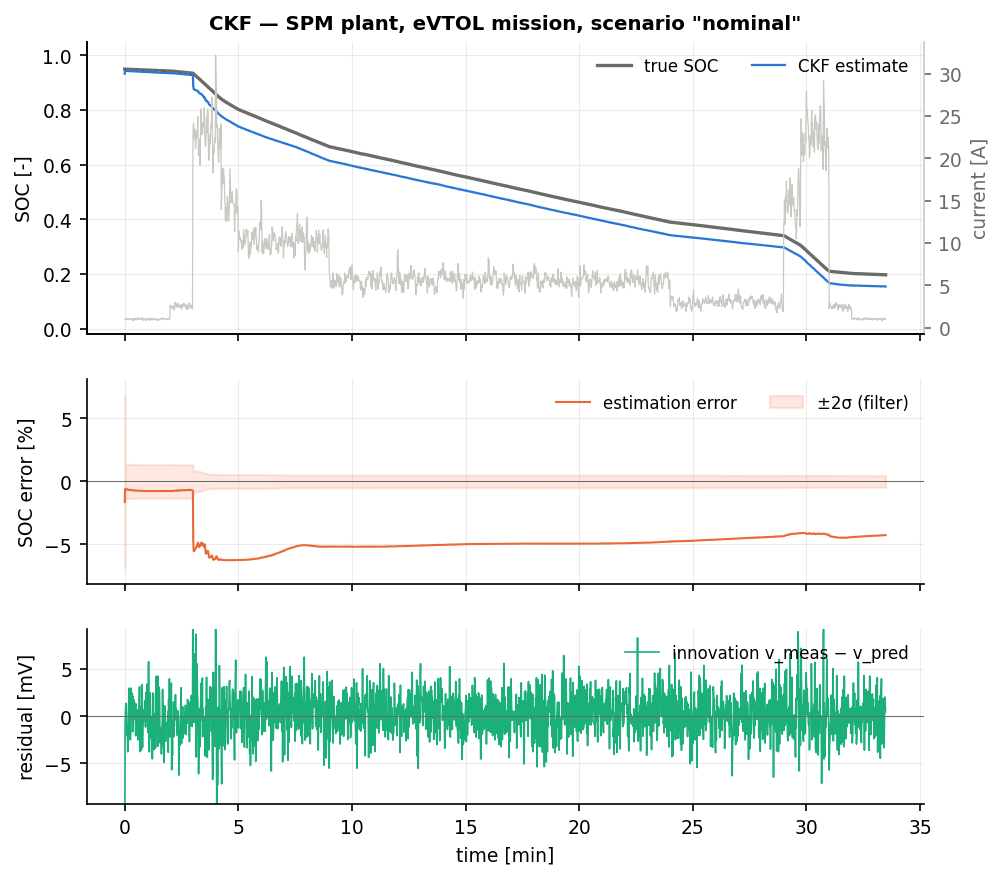
\includegraphics[width=\textwidth]{figures/cellspm_CKF_nominal.png}
\caption{CKF on the nominal mission with the electrochemical (SPM) plant.}
\end{figure}
The SPM block of the table is a different kind of test. The plant is the electrochemical
single-particle model; the estimator still runs a 2-RC equivalent circuit, fitted to that plant,
which leaves a \emph{structured} residual of about $4$\,mV (Butler--Volmer kinetics and
solid-phase diffusion that no 2-RC circuit can reproduce) and a slow second branch,
$\tau_2 = 556$\,s. Over a $33$-minute mission a $556$\,s pole barely relaxes, so $v_2(t)$ is
close to an affine ramp --- and so is $\ocv(\soc(t))$ while the cell discharges at a roughly
constant rate. The two channels through which the measurement sees the state,
$(\partial\ocv/\partial\soc)\,\delta\soc$ and $-\delta v_2$, are therefore nearly collinear in
the information accumulated over the flight: the pair $(\soc, v_2)$ is close to unobservable,
and no filter can decide whether a persistent few-millivolt residual belongs to the slow RC
branch or to the state of charge. Because that direction is weakly observable, a $4$\,mV
structured error maps onto \emph{several per cent} of SOC instead of the
$4\,\text{mV}/0.8\,\text{V}\approx0.5\,\%$ a well-conditioned channel would give. This
$(\soc,v_2)$ ambiguity, not the size of the residual, is the mechanism behind the
$3.7$--$4.6\,\%$ band in which the whole classical family sits.

The cubature filters are the \emph{worst} of the family here: $4.62\,\%$ on SPM
\texttt{nominal} against the EKF's $3.73\,\%$ and the LKF's $1.72\,\%$, $8.72\,\%$ on
\texttt{cold} against $7.35\,\%$, $8.24\,\%$ on \texttt{sensor\_dropout} against $5.31\,\%$ and
$4.81\,\%$ on \texttt{param\_mismatch} against $3.13\,\%$. The ordering across the whole family
is in fact monotone in the sigma-point spread --- LKF (frozen tangent) $1.72$, EKF/IEKF
(tangent at the mean) $3.66$--$3.73$, UKF ($0.2\sigma$ points) $3.96$, cubature filters
($2\sigma$ or $2.45\sigma$ points) $4.61$--$4.62$ --- and the ambiguity argument explains it.
A statistical linearisation taken over a wide prior returns the \emph{chord} of the OCV curve,
which is steeper than the tangent over most of the mission, so the filter believes the OCV
channel is more informative than it is and commits harder to the direction that carries the
structured error. The single exception is \texttt{outliers} ($2.21\,\%$), where every filter
does better on SPM than on ECM because the corrupted samples widen the effective innovation
covariance. Nothing diverges and $t_{\text{conv}} = 0$ on every SPM row: the error is a bias,
not a drift.

\section{Summary}
The CKF is the sigma-point filter to reach for when you want no tuning parameters and a
provably positive semi-definite covariance: it is cheaper than the UKF
($1.18$--$1.26\,\SI{}{\micro\second}$ against $1.34$--$1.46$), derivative-free, and on this
benchmark the most accurate filter of all under nominal ECM conditions. Its weakness is the
fixed $\pm\sqrt{n_x}\sigma$ point spread, which makes the statistical linearisation use the
chord rather than the tangent of a curved measurement function; with a wide prior (large
initial SOC error, sensor dropout, strong model mismatch) it converges noticeably more slowly
than an EKF, is the worst of the family on \texttt{sensor\_dropout}, and is the worst of the
family on the SPM plant. Use the square-root form (Chapter~\ref{ch:sckf}) in single precision
and the fifth-degree form (Chapter~\ref{ch:ckf5}) when the prior is wide.
